\documentclass[journal,12pt,twocolumn]{IEEEtran}

\usepackage{setspace}
\usepackage{gensymb}
\singlespacing
\usepackage[cmex10]{amsmath}
\usepackage{amssymb}
\usepackage{xurl}

\usepackage{amsthm}
\usepackage{comment}
\usepackage{mathrsfs}
\usepackage{txfonts}
\usepackage{stfloats}
\usepackage{bm}
\usepackage{cite}
\usepackage{cases}
\usepackage{subfig}

\usepackage{longtable}
\usepackage{multirow}
\usepackage{float}
\usepackage{enumitem}
\usepackage{mathtools}
\usepackage{steinmetz}
\usepackage{tikz}
\usepackage{circuitikz}
\usepackage{verbatim}
\usepackage{tfrupee}
\usepackage[breaklinks=true]{hyperref}
\usepackage{graphicx}
\usepackage{tkz-euclide}

\usetikzlibrary{calc,math}
\usepackage{listings}
    \usepackage{color}                                            %%
    \usepackage{array}                                            %%
    \usepackage{longtable}                                        %%
    \usepackage{calc}                                             %%
    \usepackage{multirow}                                         %%
    \usepackage{hhline}                                           %%
    \usepackage{ifthen}                                           %%
    \usepackage{lscape}     
\usepackage{multicol}
\usepackage{chngcntr}

\DeclareMathOperator*{\Res}{Res}

\renewcommand\thesection{\arabic{section}}
\renewcommand\thesubsection{\thesection.\arabic{subsection}}
\renewcommand\thesubsubsection{\thesubsection.\arabic{subsubsection}}

\renewcommand\thesectiondis{\arabic{section}}
\renewcommand\thesubsectiondis{\thesectiondis.\arabic{subsection}}
\renewcommand\thesubsubsectiondis{\thesubsectiondis.\arabic{subsubsection}}


\hyphenation{op-tical net-works semi-conduc-tor}
\def\inputGnumericTable{}                                 %%

\lstset{
%language=C,
frame=single, 
breaklines=true,
columns=fullflexible
}
\begin{document}


\newtheorem{theorem}{Theorem}[section]
\newtheorem{problem}{Problem}
\newtheorem{proposition}{Proposition}[section]
\newtheorem{lemma}{Lemma}[section]
\newtheorem{corollary}[theorem]{Corollary}
\newtheorem{example}{Example}[section]
\newtheorem{definition}[problem]{Definition}

\newcommand{\BEQA}{\begin{eqnarray}}
\newcommand{\EEQA}{\end{eqnarray}}
\newcommand{\define}{\stackrel{\triangle}{=}}
\bibliographystyle{IEEEtran}
\raggedbottom
\setlength{\parindent}{0pt}
\providecommand{\mbf}{\mathbf}
\providecommand{\pr}[1]{\ensuremath{\Pr\left(#1\right)}}
\providecommand{\qfunc}[1]{\ensuremath{Q\left(#1\right)}}
\providecommand{\sbrak}[1]{\ensuremath{{}\left[#1\right]}}
\providecommand{\lsbrak}[1]{\ensuremath{{}\left[#1\right.}}
\providecommand{\rsbrak}[1]{\ensuremath{{}\left.#1\right]}}
\providecommand{\brak}[1]{\ensuremath{\left(#1\right)}}
\providecommand{\lbrak}[1]{\ensuremath{\left(#1\right.}}
\providecommand{\rbrak}[1]{\ensuremath{\left.#1\right)}}
\providecommand{\cbrak}[1]{\ensuremath{\left\{#1\right\}}}
\providecommand{\lcbrak}[1]{\ensuremath{\left\{#1\right.}}
\providecommand{\rcbrak}[1]{\ensuremath{\left.#1\right\}}}
\theoremstyle{remark}
\newtheorem{rem}{Remark}
\newcommand{\sgn}{\mathop{\mathrm{sgn}}}
\providecommand{\abs}[1]{\vert#1\vert}
\providecommand{\res}[1]{\Res\displaylimits_{#1}} 
\providecommand{\norm}[1]{\lVert#1\rVert}
%\providecommand{\norm}[1]{\lVert#1\rVert}
\providecommand{\mtx}[1]{\mathbf{#1}}
\providecommand{\mean}[1]{E[ #1 ]}
\providecommand{\fourier}{\overset{\mathcal{F}}{ \rightleftharpoons}}
%\providecommand{\hilbert}{\overset{\mathcal{H}}{ \rightleftharpoons}}
\providecommand{\system}{\overset{\mathcal{H}}{ \longleftrightarrow}}
	%\newcommand{\solution}[2]{\textbf{Solution:}{#1}}
\newcommand{\solution}{\noindent \textbf{Solution: }}
\newcommand{\cosec}{\,\text{cosec}\,}
\providecommand{\dec}[2]{\ensuremath{\overset{#1}{\underset{#2}{\gtrless}}}}
\newcommand{\myvec}[1]{\ensuremath{\begin{pmatrix}#1\end{pmatrix}}}
\newcommand{\mydet}[1]{\ensuremath{\begin{vmatrix}#1\end{vmatrix}}}
\numberwithin{equation}{subsection}
\makeatletter
\@addtoreset{figure}{problem}
\makeatother
\let\StandardTheFigure\thefigure
\let\vec\mathbf
\renewcommand{\thefigure}{\theproblem}
\def\putbox#1#2#3{\makebox[0in][l]{\makebox[#1][l]{}\raisebox{\baselineskip}[0in][0in]{\raisebox{#2}[0in][0in]{#3}}}}
     \def\rightbox#1{\makebox[0in][r]{#1}}
     \def\centbox#1{\makebox[0in]{#1}}
     \def\topbox#1{\raisebox{-\baselineskip}[0in][0in]{#1}}
     \def\midbox#1{\raisebox{-0.5\baselineskip}[0in][0in]{#1}}
\vspace{3cm}
\title{ Assignment 3}
\author{Savarana Datta - AI20BTECH11008}
\maketitle
\newpage
\bigskip
\renewcommand{\thefigure}{\theenumi}
\renewcommand{\thetable}{\theenumi}
Download all python codes from 
\begin{lstlisting}
https://github.com/SavaranaDatta/EE3900/tree/main/Assignment3/codes
\end{lstlisting}
%
and latex codes from 
%
\begin{lstlisting}
https://github.com/SavaranaDatta/EE3900/tree/main/Assignment3/Assignment3.tex
\end{lstlisting}


\section{Construction 2.16}
Let ABC be a right triangle in which a=8 , c=6 and $\angle B = 90 \degree$. BD is the perpendicular from $\vec{B}$ on AC (altitude). The circle through $\vec{B},\vec{C},\vec{D}$( circumcircle of $\Delta$BCD ) is drawn. Construct the tangents from $\vec{A}$ to this circle.

\section{Solution(Construction 2.16)}
From pythagorean theorem,
\begin{align}
    b & = \sqrt{a^2+c^2}\\
      & = \sqrt{8^{2}+6^{2}}\\
      & = 10
\end{align}
Let
\begin{align}
    \vec{B} = \myvec{0\\0}\\
    \vec{C} = \myvec{a\\0}\\
    \implies \vec{C}=\myvec{8\\0}
\end{align}
The vertex $\vec{A}$ can be expressed in polar coordinate form as
\begin{align}
    \vec{A} = c\myvec{cos\theta\\sin\theta}
\end{align}
where $\angle B = \theta$
\begin{align}
    \implies \vec{A}=6\myvec{cos(90\degree)\\sin(90\degree)}\\
    \vec{A}=6\myvec{0\\1}\\
    \vec{A}=\myvec{0\\6}
\end{align}

Given BD is perpendicular from \vec{B} on AC,\\
Equation of line AC 
\begin{align}
\label{eq1}
    \frac{x}{8}+\frac{y}{6}=1 \implies \myvec{3 & 4}\vec{x}=24
\end{align}
Equation of line passing though origin and perpendicular to AC 
\begin{align}
\label{eq2}
    4x-3y=0 \implies \myvec{4 & -3}\vec{x}=0
\end{align}
The required point \vec{D} is the point of intersection of the equations \ref{eq1} and \ref{eq2}. Now we need to solve the following matrix equation
\begin{align}
    \myvec{3&4\\4&-3}\vec{x} = \myvec{24 \\0} 
\end{align}
The augmented matrix for the above equation is row reduced as follows
\begin{align}
    \myvec{3 & 4 & 24\\4 & -3 & 0} \xleftrightarrow{\text{$R_2$}\rightarrow{\text{$4R_1-3R_2$}}} \myvec{3&4&24\\0&25&96}\\
    \xleftrightarrow{\text{$R_1$}\rightarrow{\text{$R_1-\frac{4}{25}R_2$}}} \myvec{3 & 0 & \frac{216}{25}\\ 0 & 25 & 96}\\
    \implies \vec{x}=\vec{D}= \myvec{\frac{72}{25}\\\frac{96}{25}}
\end{align}
\begin{figure}[H]
   \centering
   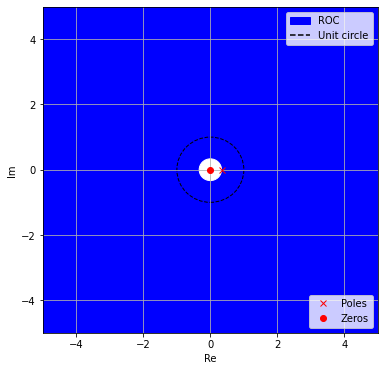
\includegraphics[width=\columnwidth]{fig1.png}
   \caption{The plot of altitude from B }
 \end{figure}
As $\Delta$BCD is right angled at D, the centre of the circumcircle is the midpoint of hypotenuse(BC) and diametre of the circumcircle is equal to length of hypotenuse(a). So,
the equation of circumcircle is
\begin{align}
\label{eq1}
    \vec{x}^\top\vec{x}-\myvec{8&0}\vec{x} = 0
\end{align}
\begin{figure}[H]
   \centering
   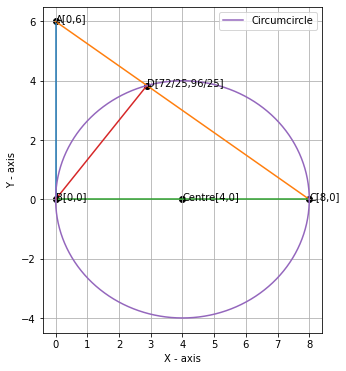
\includegraphics[width=\columnwidth]{fig2.png}
   \caption{The plot of circumcircle of $\Delta BCD$}
\end{figure}
The general equation of a secound degree can be expressed as 
\begin{align}
\label{eq2}
    \vec{x}^\top\vec{V}\vec{x}+ 2\vec{u}^\top\vec{x}+f=0
\end{align}

We know that for a circle,
\begin{align}
    \vec{V}&=\vec{I}\\
    \vec{c}&=-\vec{u}
\end{align}

Comparing the equations \ref{eq1} and \ref{eq2} we get
\begin{align}
    \vec{u}&=\myvec{-4\\0},f=0\\
    \vec{c}&=\myvec{4\\0}
\end{align}
Where $\vec{c}$ is the centre of the circumcircle.\\
The radius(r) of the circle is given by,
\begin{align}
    r & = \sqrt{\norm{c}^{2}-f}\\
      & = 4
\end{align}
Let the equation of the tangent be 
\begin{align}
\label{eq3}
    \myvec{1&m}\vec{x} = t
\end{align}
As the required tangent passes through $\vec{A}$
\begin{align}
    \myvec{1&m}\myvec{0\\6}&=t\\
    t&=6m
    \label{eq4}
\end{align}
As the perpendicular distance of the tangent from the centre of the circle is equal to the radius 
\begin{align}
    \left|{\frac{\myvec{1&m}\vec{c}-t}{\norm{\myvec{m&-1}}}}\right|&=r\\
    \left|\frac{4-6m}{\sqrt{1+m^{2}}}\right|&=4
\end{align}
Squaring on both sides
\begin{align}
    (2-3m)^{2}&=4+4m^{2}\\
    5m^{2}&=12m\\
    m&=\frac{12}{5} (or)\\
    m&=0
\end{align}
From equation \ref{eq3} and \ref{eq4}, we can conclude that the lines $\myvec{1&\frac{12}{5}}\vec{x}=\frac{72}{5}$ and $\myvec{1&0}\vec{x}=0$ are tangents from vertex $\vec{A}$ to the circumcircle of $\Delta BCD$ 
\begin{figure}[!ht]
   \centering
   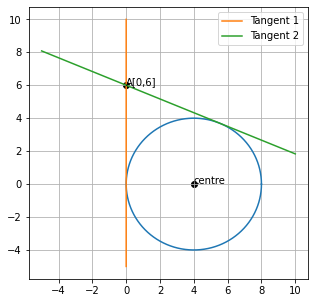
\includegraphics[width=\columnwidth]{fig3.png}
   \caption{The plots of tangents to the circle}
\end{figure}


\end{document}


